\begin{frame}
\frametitle{UI Consistency}
Many teams, many components. How to manage this mess?
\pause
\begin{figure}
	\centering
	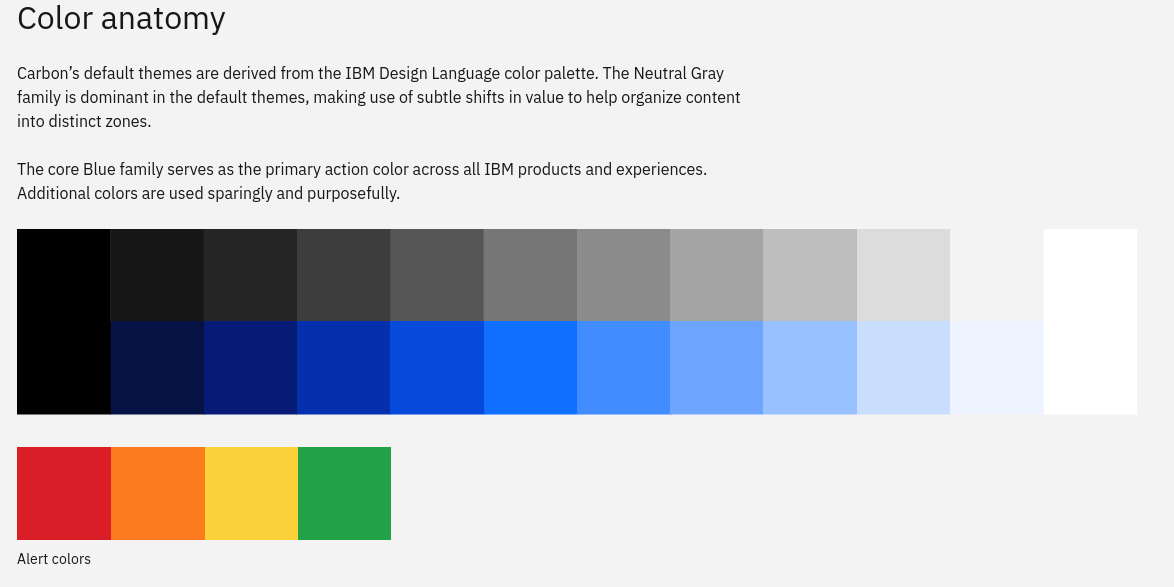
\includegraphics[width=0.7\linewidth]{pictures/ibm-color}
	\caption{IBM - color anatomy}
	\label{fig:ibm-color}
\end{figure}


\end{frame}


\begin{frame}
\frametitle{UI Consistency}

\begin{figure}
	\centering
	
\includegraphics[width=0.7\linewidth]{pictures/design-MATERIAL.png}
	\caption{Material UI - menu height}
	\label{fig:material-UI}
\end{figure}


\end{frame}